\documentclass[letterpaper, 24pt, final, onecolumn, titlepage] {article}

\usepackage{enumerate}
\usepackage{graphicx}
\usepackage{listings}
\usepackage{color}
\usepackage{setspace}
\usepackage {amsmath}
\usepackage{amssymb}

\title{ECE 270: Computer Methods in ECE \\
	\vspace{1.5cm}
   		\begin{center}\includegraphics{umlogo} \end{center}
	\vspace{1.5cm}
	\textbf{Quiz \#3} \\
	Random Walk}
	
\author{Hussein El-Souri}

\date{\today}

\definecolor{dkgreen}{rgb}{0,0.6,0}
\definecolor{gray}{rgb}{0.5,0.5,0.5}
\definecolor{mauve}{rgb}{0.58,0,0.82}

\lstset{frame=tb,
  language=C,
  aboveskip=3mm,
  belowskip=3mm,
  showstringspaces=false,
  columns=flexible,
  basicstyle={\small\ttfamily},
  numbers=none,
  numberstyle=\tiny\color{gray},
  keywordstyle=\color{blue},
  commentstyle=\color{dkgreen},
  stringstyle=\color{mauve},
  breaklines=true,
  breakatwhitespace=true,
  tabsize=3
}

\begin{document}

\maketitle

\doublespacing

\section{Testing and Output}

\begin{center}\includegraphics{screen1} \end{center}
\pagebreak
\begin{center}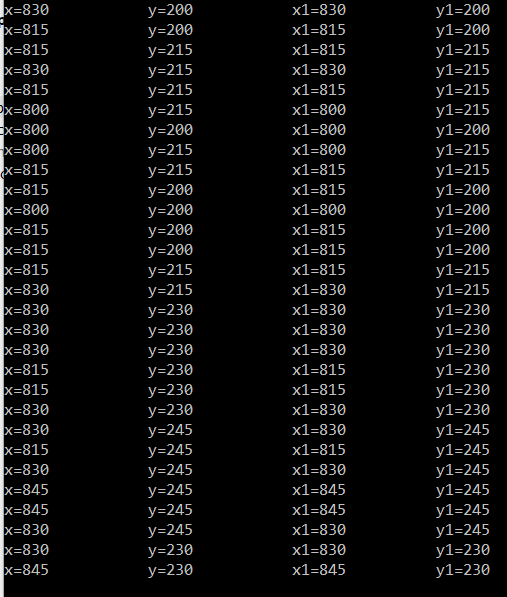
\includegraphics{screen2} \end{center}
\pagebreak
\section{Code}
\singlespacing

\begin{lstlisting}

//----------changes made to ofApp.h-------------//
class ofApp : public ofBaseApp{
	public:
	    int x,y,x1,y1;
	    int RandSign()
	    {
	        int sign;
	        sign = rand()%2;
	        if(sign ==0) sign=-1;
	        return sign;
	    }
	    int ChangeColor()
	    {
	        int ColorValue;
	        ColorValue = 1 + rand()%256; //to return a random value of RGB between 1 and 255
                                        //i skipped the RGB value 0 0 0 because it gives black and background is black :)
	        return ColorValue;
	    }
		void setup();
		void update();
		void draw();
		void keyPressed(int key);
		void keyReleased(int key);
		void mouseMoved(int x, int y);
		void mouseDragged(int x, int y, int button);
		void mousePressed(int x, int y, int button);
		void mouseReleased(int x, int y, int button);
		void windowResized(int w, int h);
		void dragEvent(ofDragInfo dragInfo);
		void gotMessage(ofMessage msg);
};

//----------changes made to ofApp.cpp-------------//
void ofApp::setup(){
    x=500; y=500;
    x1=500; y1=500;
    ofBackground(0,0,0);
    ofSetBackgroundAuto(false);
    ofSetFrameRate(50);
}
//--------------------------------------------------------------
void ofApp::update(){
    printf("x=%d\t\ty=%d\t\tx1=%d\t\ty1=%d\n",x,y,x1,y1);
    if (rand()%2==0) x1+=RandSign()*15;
    else if(rand()%2==1) y1+=RandSign()*15;
}
//--------------------------------------------------------------
void ofApp::draw(){
    ofSetColor(ChangeColor(),ChangeColor(),ChangeColor());
    ofLine(x,y,x1,y1);
    x=x1; y=y1;
}
//---------------------------------------------------//
\end{lstlisting}


\end{document}